\documentclass[twoside]{book}

% Packages required by doxygen
\usepackage{calc}
\usepackage{doxygen}
\usepackage{graphicx}
\usepackage[utf8]{inputenc}
\usepackage{makeidx}
\usepackage{multicol}
\usepackage{multirow}
\usepackage{textcomp}
\usepackage[table]{xcolor}

% Font selection
\usepackage[T1]{fontenc}
\usepackage{mathptmx}
\usepackage[scaled=.90]{helvet}
\usepackage{courier}
\usepackage{amssymb}
\usepackage{sectsty}
\renewcommand{\familydefault}{\sfdefault}
\allsectionsfont{%
  \fontseries{bc}\selectfont%
  \color{darkgray}%
}
\renewcommand{\DoxyLabelFont}{%
  \fontseries{bc}\selectfont%
  \color{darkgray}%
}

% Page & text layout
\usepackage{geometry}
\geometry{%
  a4paper,%
  top=2.5cm,%
  bottom=2.5cm,%
  left=2.5cm,%
  right=2.5cm%
}
\tolerance=750
\hfuzz=15pt
\hbadness=750
\setlength{\emergencystretch}{15pt}
\setlength{\parindent}{0cm}
\setlength{\parskip}{0.2cm}
\makeatletter
\renewcommand{\paragraph}{%
  \@startsection{paragraph}{4}{0ex}{-1.0ex}{1.0ex}{%
    \normalfont\normalsize\bfseries\SS@parafont%
  }%
}
\renewcommand{\subparagraph}{%
  \@startsection{subparagraph}{5}{0ex}{-1.0ex}{1.0ex}{%
    \normalfont\normalsize\bfseries\SS@subparafont%
  }%
}
\makeatother

% Headers & footers
\usepackage{fancyhdr}
\pagestyle{fancyplain}
\fancyhead[LE]{\fancyplain{}{\bfseries\thepage}}
\fancyhead[CE]{\fancyplain{}{}}
\fancyhead[RE]{\fancyplain{}{\bfseries\leftmark}}
\fancyhead[LO]{\fancyplain{}{\bfseries\rightmark}}
\fancyhead[CO]{\fancyplain{}{}}
\fancyhead[RO]{\fancyplain{}{\bfseries\thepage}}
\fancyfoot[LE]{\fancyplain{}{}}
\fancyfoot[CE]{\fancyplain{}{}}
\fancyfoot[RE]{\fancyplain{}{\bfseries\scriptsize Generated on Tue Feb 11 2014 12\-:57\-:58 for Chess Game by Doxygen }}
\fancyfoot[LO]{\fancyplain{}{\bfseries\scriptsize Generated on Tue Feb 11 2014 12\-:57\-:58 for Chess Game by Doxygen }}
\fancyfoot[CO]{\fancyplain{}{}}
\fancyfoot[RO]{\fancyplain{}{}}
\renewcommand{\footrulewidth}{0.4pt}
\renewcommand{\chaptermark}[1]{%
  \markboth{#1}{}%
}
\renewcommand{\sectionmark}[1]{%
  \markright{\thesection\ #1}%
}

% Indices & bibliography
\usepackage{natbib}
\usepackage[titles]{tocloft}
\setcounter{tocdepth}{3}
\setcounter{secnumdepth}{5}
\makeindex

% Hyperlinks (required, but should be loaded last)
\usepackage{ifpdf}
\ifpdf
  \usepackage[pdftex,pagebackref=true]{hyperref}
\else
  \usepackage[ps2pdf,pagebackref=true]{hyperref}
\fi
\hypersetup{%
  colorlinks=true,%
  linkcolor=blue,%
  citecolor=blue,%
  unicode%
}

% Custom commands
\newcommand{\clearemptydoublepage}{%
  \newpage{\pagestyle{empty}\cleardoublepage}%
}


%===== C O N T E N T S =====

\begin{document}

% Titlepage & ToC
\hypersetup{pageanchor=false}
\pagenumbering{roman}
\begin{titlepage}
\vspace*{7cm}
\begin{center}%
{\Large Chess Game }\\
\vspace*{1cm}
{\large Generated by Doxygen 1.8.6}\\
\vspace*{0.5cm}
{\small Tue Feb 11 2014 12:57:58}\\
\end{center}
\end{titlepage}
\clearemptydoublepage
\tableofcontents
\clearemptydoublepage
\pagenumbering{arabic}
\hypersetup{pageanchor=true}

%--- Begin generated contents ---
\chapter{Namespace Index}
\section{Packages}
Here are the packages with brief descriptions (if available)\-:\begin{DoxyCompactList}
\item\contentsline{section}{\hyperlink{namespace_basic___objects}{Basic\-\_\-\-Objects} }{\pageref{namespace_basic___objects}}{}
\item\contentsline{section}{\hyperlink{namespace_movement_test}{Movement\-Test} }{\pageref{namespace_movement_test}}{}
\end{DoxyCompactList}

\chapter{Hierarchical Index}
\section{Class Hierarchy}
This inheritance list is sorted roughly, but not completely, alphabetically\-:\begin{DoxyCompactList}
\item \contentsline{section}{Chess\-Game\-Demo\-Test}{\pageref{class_chess_game_demo_test}}{}
\item \contentsline{section}{Game}{\pageref{class_game}}{}
\item J\-Frame\begin{DoxyCompactList}
\item \contentsline{section}{Chess\-Game\-Demo}{\pageref{class_chess_game_demo}}{}
\end{DoxyCompactList}
\item Mouse\-Listener\begin{DoxyCompactList}
\item \contentsline{section}{Chess\-Game\-Demo}{\pageref{class_chess_game_demo}}{}
\end{DoxyCompactList}
\item Mouse\-Motion\-Listener\begin{DoxyCompactList}
\item \contentsline{section}{Chess\-Game\-Demo}{\pageref{class_chess_game_demo}}{}
\end{DoxyCompactList}
\item \contentsline{section}{Movement\-Check}{\pageref{class_movement_check}}{}
\item \contentsline{section}{Movement\-Check\-Test}{\pageref{class_movement_check_test}}{}
\end{DoxyCompactList}

\chapter{Class Index}
\section{Class List}
Here are the classes, structs, unions and interfaces with brief descriptions\-:\begin{DoxyCompactList}
\item\contentsline{section}{\hyperlink{class_chess_game_demo}{Chess\-Game\-Demo} }{\pageref{class_chess_game_demo}}{}
\item\contentsline{section}{\hyperlink{class_chess_game_demo_test}{Chess\-Game\-Demo\-Test} }{\pageref{class_chess_game_demo_test}}{}
\item\contentsline{section}{\hyperlink{class_game}{Game} }{\pageref{class_game}}{}
\item\contentsline{section}{\hyperlink{class_movement_1_1_movement}{Movement.\-Movement} }{\pageref{class_movement_1_1_movement}}{}
\item\contentsline{section}{\hyperlink{class_movement_1_1_movement_bishop}{Movement.\-Movement\-Bishop} }{\pageref{class_movement_1_1_movement_bishop}}{}
\item\contentsline{section}{\hyperlink{class_movement_test_1_1_movement_bishop_test}{Movement\-Test.\-Movement\-Bishop\-Test} }{\pageref{class_movement_test_1_1_movement_bishop_test}}{}
\item\contentsline{section}{\hyperlink{class_movement_check}{Movement\-Check} }{\pageref{class_movement_check}}{}
\item\contentsline{section}{\hyperlink{class_movement_check_test}{Movement\-Check\-Test} }{\pageref{class_movement_check_test}}{}
\item\contentsline{section}{\hyperlink{class_movement_1_1_movement_king}{Movement.\-Movement\-King} }{\pageref{class_movement_1_1_movement_king}}{}
\item\contentsline{section}{\hyperlink{class_movement_test_1_1_movement_king_test}{Movement\-Test.\-Movement\-King\-Test} }{\pageref{class_movement_test_1_1_movement_king_test}}{}
\item\contentsline{section}{\hyperlink{class_movement_1_1_movement_knight}{Movement.\-Movement\-Knight} }{\pageref{class_movement_1_1_movement_knight}}{}
\item\contentsline{section}{\hyperlink{class_movement_test_1_1_movement_knight_test}{Movement\-Test.\-Movement\-Knight\-Test} }{\pageref{class_movement_test_1_1_movement_knight_test}}{}
\item\contentsline{section}{\hyperlink{class_movement_1_1_movement_pawn}{Movement.\-Movement\-Pawn} }{\pageref{class_movement_1_1_movement_pawn}}{}
\item\contentsline{section}{\hyperlink{class_movement_test_1_1_movement_pawn_test}{Movement\-Test.\-Movement\-Pawn\-Test} }{\pageref{class_movement_test_1_1_movement_pawn_test}}{}
\item\contentsline{section}{\hyperlink{class_movement_1_1_movement_rock}{Movement.\-Movement\-Rock} }{\pageref{class_movement_1_1_movement_rock}}{}
\item\contentsline{section}{\hyperlink{class_basic___objects_1_1_piece}{Basic\-\_\-\-Objects.\-Piece} }{\pageref{class_basic___objects_1_1_piece}}{}
\item\contentsline{section}{\hyperlink{class_basic___objects_1_1_position}{Basic\-\_\-\-Objects.\-Position} }{\pageref{class_basic___objects_1_1_position}}{}
\end{DoxyCompactList}

\chapter{Namespace Documentation}
\hypertarget{namespace_basic___objects}{\section{Package Basic\-\_\-\-Objects}
\label{namespace_basic___objects}\index{Basic\-\_\-\-Objects@{Basic\-\_\-\-Objects}}
}
\subsection*{Classes}
\begin{DoxyCompactItemize}
\item 
class \hyperlink{class_basic___objects_1_1_piece}{Piece}
\item 
class \hyperlink{class_basic___objects_1_1_player}{Player}
\item 
class \hyperlink{class_basic___objects_1_1_position}{Position}
\end{DoxyCompactItemize}


\subsection{Detailed Description}
\begin{DoxyAuthor}{Author}
ignacioferrero 
\end{DoxyAuthor}

\hypertarget{namespace_movement_test}{\section{Package Movement\-Test}
\label{namespace_movement_test}\index{Movement\-Test@{Movement\-Test}}
}
\subsection*{Classes}
\begin{DoxyCompactItemize}
\item 
class \hyperlink{class_movement_test_1_1_chess_game_demo_test}{Chess\-Game\-Demo\-Test}
\item 
class \hyperlink{class_movement_test_1_1_movement_bishop_test}{Movement\-Bishop\-Test}
\item 
class \hyperlink{class_movement_test_1_1_movement_king_test}{Movement\-King\-Test}
\item 
class \hyperlink{class_movement_test_1_1_movement_knight_test}{Movement\-Knight\-Test}
\item 
class \hyperlink{class_movement_test_1_1_movement_pawn_test}{Movement\-Pawn\-Test}
\end{DoxyCompactItemize}


\subsection{Detailed Description}
\begin{DoxyAuthor}{Author}
ignacioferrero 
\end{DoxyAuthor}

\chapter{Class Documentation}
\hypertarget{class_board}{\section{Board Class Reference}
\label{class_board}\index{Board@{Board}}
}
Inheritance diagram for Board\-:\begin{figure}[H]
\begin{center}
\leavevmode
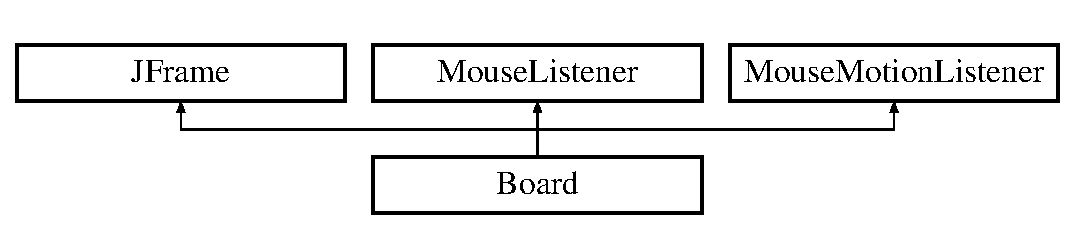
\includegraphics[height=2.000000cm]{class_board}
\end{center}
\end{figure}
\subsection*{Public Member Functions}
\begin{DoxyCompactItemize}
\item 
\hypertarget{class_board_a5fa302f692f0cd37377e8eeea570d599}{{\bfseries Board} (\hyperlink{class_game_logic}{Game\-Logic} \-\_\-game\-\_\-logic)}\label{class_board_a5fa302f692f0cd37377e8eeea570d599}

\item 
void \hyperlink{class_board_a37b7c03eacc3aec9ba48533ab3838f11}{mouse\-Pressed} (Mouse\-Event e)
\item 
void \hyperlink{class_board_ad2aee45964de8e92562032c36d7643c9}{mouse\-Dragged} (Mouse\-Event me)
\item 
void \hyperlink{class_board_abd7848e4044ed956d3b7f207f6d99ef9}{mouse\-Released} (Mouse\-Event e)
\item 
Boolean \hyperlink{class_board_a499318c478aea617ffe42f6e002f74ef}{get\-Finish} ()
\item 
void \hyperlink{class_board_a522a240b57c601ac68dae4e02022ca56}{check\-Dialog} ()
\item 
void \hyperlink{class_board_aceec202d7656676418e88bb0ac2d122d}{check\-Mate\-Dialog} ()
\item 
void \hyperlink{class_board_a0949e66b93c73ea67065a3b7c5e1bcae}{check\-Error\-Turn} ()
\item 
\hypertarget{class_board_a5bcac6239ccaccd32267bdd7045d89d7}{void {\bfseries mouse\-Clicked} (Mouse\-Event e)}\label{class_board_a5bcac6239ccaccd32267bdd7045d89d7}

\item 
\hypertarget{class_board_a683e962b3ce5f3dcdcdecf5ddddb0cbf}{void {\bfseries mouse\-Moved} (Mouse\-Event e)}\label{class_board_a683e962b3ce5f3dcdcdecf5ddddb0cbf}

\item 
\hypertarget{class_board_af0a6c48adfbfda0decef55ea852af326}{void {\bfseries mouse\-Entered} (Mouse\-Event e)}\label{class_board_af0a6c48adfbfda0decef55ea852af326}

\item 
\hypertarget{class_board_a0750ca283683f18505df7cd31653b62c}{void {\bfseries mouse\-Exited} (Mouse\-Event e)}\label{class_board_a0750ca283683f18505df7cd31653b62c}

\item 
\hypertarget{class_board_abed7b49b7504f432dd0f39e2e72714d2}{void {\bfseries window\-Closing} (Window\-Event e)}\label{class_board_abed7b49b7504f432dd0f39e2e72714d2}

\end{DoxyCompactItemize}


\subsection{Detailed Description}
Class for managing the board ,creating the G\-U\-I and handling the M\-O\-U\-S\-E -\/events independent from 

\subsection{Member Function Documentation}
\hypertarget{class_board_a522a240b57c601ac68dae4e02022ca56}{\index{Board@{Board}!check\-Dialog@{check\-Dialog}}
\index{check\-Dialog@{check\-Dialog}!Board@{Board}}
\subsubsection[{check\-Dialog}]{\setlength{\rightskip}{0pt plus 5cm}void Board.\-check\-Dialog (
\begin{DoxyParamCaption}
{}
\end{DoxyParamCaption}
)}}\label{class_board_a522a240b57c601ac68dae4e02022ca56}
Function to show check \hypertarget{class_board_a0949e66b93c73ea67065a3b7c5e1bcae}{\index{Board@{Board}!check\-Error\-Turn@{check\-Error\-Turn}}
\index{check\-Error\-Turn@{check\-Error\-Turn}!Board@{Board}}
\subsubsection[{check\-Error\-Turn}]{\setlength{\rightskip}{0pt plus 5cm}void Board.\-check\-Error\-Turn (
\begin{DoxyParamCaption}
{}
\end{DoxyParamCaption}
)}}\label{class_board_a0949e66b93c73ea67065a3b7c5e1bcae}
Function to show that is it not your turn \hypertarget{class_board_aceec202d7656676418e88bb0ac2d122d}{\index{Board@{Board}!check\-Mate\-Dialog@{check\-Mate\-Dialog}}
\index{check\-Mate\-Dialog@{check\-Mate\-Dialog}!Board@{Board}}
\subsubsection[{check\-Mate\-Dialog}]{\setlength{\rightskip}{0pt plus 5cm}void Board.\-check\-Mate\-Dialog (
\begin{DoxyParamCaption}
{}
\end{DoxyParamCaption}
)}}\label{class_board_aceec202d7656676418e88bb0ac2d122d}
Function to show check\-Mate \hypertarget{class_board_a499318c478aea617ffe42f6e002f74ef}{\index{Board@{Board}!get\-Finish@{get\-Finish}}
\index{get\-Finish@{get\-Finish}!Board@{Board}}
\subsubsection[{get\-Finish}]{\setlength{\rightskip}{0pt plus 5cm}Boolean Board.\-get\-Finish (
\begin{DoxyParamCaption}
{}
\end{DoxyParamCaption}
)}}\label{class_board_a499318c478aea617ffe42f6e002f74ef}
\hyperlink{class_game}{Game} is finished \hypertarget{class_board_ad2aee45964de8e92562032c36d7643c9}{\index{Board@{Board}!mouse\-Dragged@{mouse\-Dragged}}
\index{mouse\-Dragged@{mouse\-Dragged}!Board@{Board}}
\subsubsection[{mouse\-Dragged}]{\setlength{\rightskip}{0pt plus 5cm}void Board.\-mouse\-Dragged (
\begin{DoxyParamCaption}
\item[{Mouse\-Event}]{me}
\end{DoxyParamCaption}
)}}\label{class_board_ad2aee45964de8e92562032c36d7643c9}
Mouse pressed Event to take the initial position source from \href{http://forgetcode.com/Java/848-Chess-game-Swing}{\tt http\-://forgetcode.\-com/\-Java/848-\/\-Chess-\/game-\/\-Swing} gets the piece while dragging the piece to final position so it does not disappear \hypertarget{class_board_a37b7c03eacc3aec9ba48533ab3838f11}{\index{Board@{Board}!mouse\-Pressed@{mouse\-Pressed}}
\index{mouse\-Pressed@{mouse\-Pressed}!Board@{Board}}
\subsubsection[{mouse\-Pressed}]{\setlength{\rightskip}{0pt plus 5cm}void Board.\-mouse\-Pressed (
\begin{DoxyParamCaption}
\item[{Mouse\-Event}]{e}
\end{DoxyParamCaption}
)}}\label{class_board_a37b7c03eacc3aec9ba48533ab3838f11}
Mouse pressed Event to take the initial position source from \href{http://forgetcode.com/Java/848-Chess-game-Swing}{\tt http\-://forgetcode.\-com/\-Java/848-\/\-Chess-\/game-\/\-Swing} \hypertarget{class_board_abd7848e4044ed956d3b7f207f6d99ef9}{\index{Board@{Board}!mouse\-Released@{mouse\-Released}}
\index{mouse\-Released@{mouse\-Released}!Board@{Board}}
\subsubsection[{mouse\-Released}]{\setlength{\rightskip}{0pt plus 5cm}void Board.\-mouse\-Released (
\begin{DoxyParamCaption}
\item[{Mouse\-Event}]{e}
\end{DoxyParamCaption}
)}}\label{class_board_abd7848e4044ed956d3b7f207f6d99ef9}
Mouse pressed Event to take the initial position source from \href{http://forgetcode.com/Java/848-Chess-game-Swing}{\tt http\-://forgetcode.\-com/\-Java/848-\/\-Chess-\/game-\/\-Swing} Grabs end position to allow or disallow the move updates the board if the movement is allowed 

The documentation for this class was generated from the following file\-:\begin{DoxyCompactItemize}
\item 
src/Board.\-java\end{DoxyCompactItemize}

\hypertarget{class_movement_test_1_1_chess_game_demo_test}{\section{Movement\-Test.\-Chess\-Game\-Demo\-Test Class Reference}
\label{class_movement_test_1_1_chess_game_demo_test}\index{Movement\-Test.\-Chess\-Game\-Demo\-Test@{Movement\-Test.\-Chess\-Game\-Demo\-Test}}
}
\subsection*{Public Member Functions}
\begin{DoxyCompactItemize}
\item 
\hypertarget{class_movement_test_1_1_chess_game_demo_test_af6f4d48c1dea3eca919c1f1faa0329ab}{void {\bfseries test} ()}\label{class_movement_test_1_1_chess_game_demo_test_af6f4d48c1dea3eca919c1f1faa0329ab}

\end{DoxyCompactItemize}


The documentation for this class was generated from the following file\-:\begin{DoxyCompactItemize}
\item 
src/\-Movement\-Test/Chess\-Game\-Demo\-Test.\-java\end{DoxyCompactItemize}

\hypertarget{class_game}{\section{Game Class Reference}
\label{class_game}\index{Game@{Game}}
}
\subsection*{Static Public Member Functions}
\begin{DoxyCompactItemize}
\item 
\hypertarget{class_game_ae52595a27ac1b327b05db2129ad81fca}{static void {\bfseries main} (String\mbox{[}$\,$\mbox{]} args)}\label{class_game_ae52595a27ac1b327b05db2129ad81fca}

\end{DoxyCompactItemize}


The documentation for this class was generated from the following file\-:\begin{DoxyCompactItemize}
\item 
Game.\-java\end{DoxyCompactItemize}

\hypertarget{class_game_logic}{\section{Game\-Logic Class Reference}
\label{class_game_logic}\index{Game\-Logic@{Game\-Logic}}
}
\subsection*{Public Member Functions}
\begin{DoxyCompactItemize}
\item 
\hypertarget{class_game_logic_ab3a9a378dc6771bf80787eb3f7813e49}{void {\bfseries update\-Player} (\hyperlink{class_basic___objects_1_1_player}{Player} \-\_\-p)}\label{class_game_logic_ab3a9a378dc6771bf80787eb3f7813e49}

\item 
\hypertarget{class_game_logic_a281db5c4df0f5d9c7a0a42a029fb79cf}{void {\bfseries update\-App} ()}\label{class_game_logic_a281db5c4df0f5d9c7a0a42a029fb79cf}

\item 
\hypertarget{class_game_logic_a77f8b1d5fad85c98ef3b562d138761dd}{boolean {\bfseries getupdate\-App} ()}\label{class_game_logic_a77f8b1d5fad85c98ef3b562d138761dd}

\item 
\hypertarget{class_game_logic_a16750c53bed78409f51cc8531f87728c}{boolean {\bfseries update} (\hyperlink{class_basic___objects_1_1_position}{Position} \-\_\-init, \hyperlink{class_basic___objects_1_1_position}{Position} \-\_\-end)}\label{class_game_logic_a16750c53bed78409f51cc8531f87728c}

\item 
\hypertarget{class_game_logic_a51098caf4637d2cf22564ffd4240833c}{boolean {\bfseries Game\-Finished} ()}\label{class_game_logic_a51098caf4637d2cf22564ffd4240833c}

\item 
\hypertarget{class_game_logic_a18199d3792eaa46a205c80e899cb2f5d}{boolean {\bfseries movement\-Complete} ()}\label{class_game_logic_a18199d3792eaa46a205c80e899cb2f5d}

\item 
\hypertarget{class_game_logic_a9f71589900e8f80b7d67091144cc7c39}{boolean {\bfseries check\-Mate} ()}\label{class_game_logic_a9f71589900e8f80b7d67091144cc7c39}

\end{DoxyCompactItemize}


The documentation for this class was generated from the following file\-:\begin{DoxyCompactItemize}
\item 
src/Game\-Logic.\-java\end{DoxyCompactItemize}

\hypertarget{class_movement_1_1_movement}{\section{Movement.\-Movement Class Reference}
\label{class_movement_1_1_movement}\index{Movement.\-Movement@{Movement.\-Movement}}
}
Inheritance diagram for Movement.\-Movement\-:\begin{figure}[H]
\begin{center}
\leavevmode
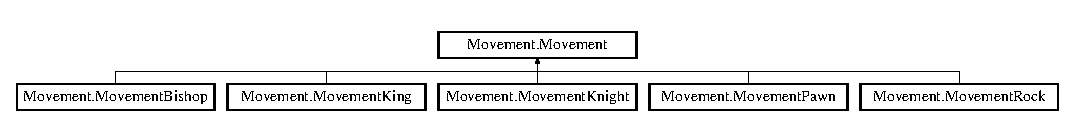
\includegraphics[height=1.258427cm]{class_movement_1_1_movement}
\end{center}
\end{figure}
\subsection*{Protected Member Functions}
\begin{DoxyCompactItemize}
\item 
\hypertarget{class_movement_1_1_movement_a74f7e5fbbc387323a207153cd994cc12}{boolean {\bfseries checkoutofbounds} (int i, int j)}\label{class_movement_1_1_movement_a74f7e5fbbc387323a207153cd994cc12}

\item 
\hypertarget{class_movement_1_1_movement_a8ac847fe5ca8f8069ed9967a67443dee}{boolean {\bfseries check\-Colorempty} (int i, int j)}\label{class_movement_1_1_movement_a8ac847fe5ca8f8069ed9967a67443dee}

\end{DoxyCompactItemize}


The documentation for this class was generated from the following file\-:\begin{DoxyCompactItemize}
\item 
src/\-Movement/Movement.\-java\end{DoxyCompactItemize}

\hypertarget{class_movement_1_1_movement_bishop}{\section{Movement.\-Movement\-Bishop Class Reference}
\label{class_movement_1_1_movement_bishop}\index{Movement.\-Movement\-Bishop@{Movement.\-Movement\-Bishop}}
}
Inheritance diagram for Movement.\-Movement\-Bishop\-:\begin{figure}[H]
\begin{center}
\leavevmode
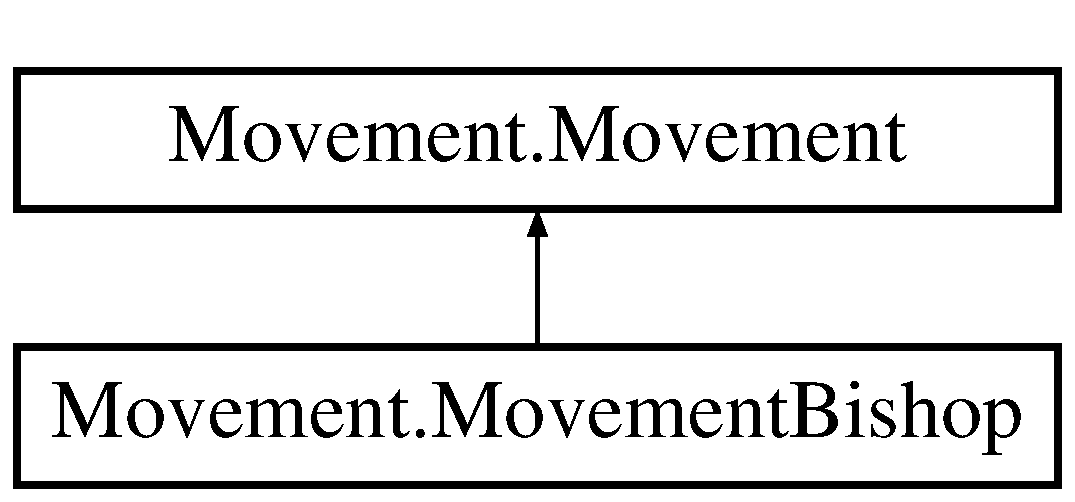
\includegraphics[height=2.000000cm]{class_movement_1_1_movement_bishop}
\end{center}
\end{figure}
\subsection*{Public Member Functions}
\begin{DoxyCompactItemize}
\item 
\hypertarget{class_movement_1_1_movement_bishop_a783880ac01ad8ed6f877881b2d9d255c}{{\bfseries Movement\-Bishop} (\hyperlink{class_basic___objects_1_1_piece}{Piece}\mbox{[}$\,$\mbox{]}\mbox{[}$\,$\mbox{]} \-\_\-pieces, \hyperlink{class_basic___objects_1_1_piece}{Piece} \-\_\-piece, int \-\_\-x, int \-\_\-y)}\label{class_movement_1_1_movement_bishop_a783880ac01ad8ed6f877881b2d9d255c}

\item 
Array\-List$<$ \hyperlink{class_basic___objects_1_1_position}{Position} $>$ \hyperlink{class_movement_1_1_movement_bishop_a11339825d69b3b9c404644b6ae9200a6}{check\-Bishop} ()
\end{DoxyCompactItemize}
\subsection*{Protected Member Functions}
\begin{DoxyCompactItemize}
\item 
\hypertarget{class_movement_1_1_movement_bishop_a36fde142cd1c4810e2577a744f736687}{boolean\mbox{[}$\,$\mbox{]} {\bfseries check\-Movement} (int i, int j)}\label{class_movement_1_1_movement_bishop_a36fde142cd1c4810e2577a744f736687}

\end{DoxyCompactItemize}


\subsection{Detailed Description}
\hyperlink{class_movement_1_1_movement_rock}{Movement\-Rock} , control the Movements of the Bishop \begin{DoxyAuthor}{Author}
Ignacio Ferrero 
\end{DoxyAuthor}


\subsection{Member Function Documentation}
\hypertarget{class_movement_1_1_movement_bishop_a11339825d69b3b9c404644b6ae9200a6}{\index{Movement\-::\-Movement\-Bishop@{Movement\-::\-Movement\-Bishop}!check\-Bishop@{check\-Bishop}}
\index{check\-Bishop@{check\-Bishop}!Movement::MovementBishop@{Movement\-::\-Movement\-Bishop}}
\subsubsection[{check\-Bishop}]{\setlength{\rightskip}{0pt plus 5cm}Array\-List$<${\bf Position}$>$ Movement.\-Movement\-Bishop.\-check\-Bishop (
\begin{DoxyParamCaption}
{}
\end{DoxyParamCaption}
)}}\label{class_movement_1_1_movement_bishop_a11339825d69b3b9c404644b6ae9200a6}
Gives back every available \hyperlink{class_movement_1_1_movement}{Movement} that the Bishop has with a for that expands like an X 

The documentation for this class was generated from the following file\-:\begin{DoxyCompactItemize}
\item 
src/\-Movement/Movement\-Bishop.\-java\end{DoxyCompactItemize}

\hypertarget{class_movement_test_1_1_movement_bishop_test}{\section{Movement\-Test.\-Movement\-Bishop\-Test Class Reference}
\label{class_movement_test_1_1_movement_bishop_test}\index{Movement\-Test.\-Movement\-Bishop\-Test@{Movement\-Test.\-Movement\-Bishop\-Test}}
}
\subsection*{Public Member Functions}
\begin{DoxyCompactItemize}
\item 
\hypertarget{class_movement_test_1_1_movement_bishop_test_a93a4a3c215e76e1375be38853ca4a0a2}{void {\bfseries test\-Check\-Bishop} ()}\label{class_movement_test_1_1_movement_bishop_test_a93a4a3c215e76e1375be38853ca4a0a2}

\item 
\hypertarget{class_movement_test_1_1_movement_bishop_test_a4d5a76dde27feb3496d45d36d377f130}{void {\bfseries create\-Piece\-Correct} ()}\label{class_movement_test_1_1_movement_bishop_test_a4d5a76dde27feb3496d45d36d377f130}

\item 
\hypertarget{class_movement_test_1_1_movement_bishop_test_a862c0caeae649e7a3a454a441f86aba0}{void {\bfseries create\-Piece\-Incorrect} ()}\label{class_movement_test_1_1_movement_bishop_test_a862c0caeae649e7a3a454a441f86aba0}

\item 
\hypertarget{class_movement_test_1_1_movement_bishop_test_adcb77e9441c7ef262ed6ec8695a7b3b9}{void {\bfseries initialize} ()}\label{class_movement_test_1_1_movement_bishop_test_adcb77e9441c7ef262ed6ec8695a7b3b9}

\end{DoxyCompactItemize}


The documentation for this class was generated from the following file\-:\begin{DoxyCompactItemize}
\item 
src/\-Movement\-Test/Movement\-Bishop\-Test.\-java\end{DoxyCompactItemize}

\hypertarget{class_movement_check}{\section{Movement\-Check Class Reference}
\label{class_movement_check}\index{Movement\-Check@{Movement\-Check}}
}
\subsection*{Public Member Functions}
\begin{DoxyCompactItemize}
\item 
\hypertarget{class_movement_check_ad4282505567223574aad557238ec3962}{void {\bfseries update} (\hyperlink{class_basic___objects_1_1_piece}{Piece}\mbox{[}$\,$\mbox{]}\mbox{[}$\,$\mbox{]} \-\_\-pieces)}\label{class_movement_check_ad4282505567223574aad557238ec3962}

\item 
\hypertarget{class_movement_check_a7de16c5e5e34bea53f45a84c0357b3cf}{boolean {\bfseries check\-Move} (\hyperlink{class_basic___objects_1_1_piece}{Piece} p, \hyperlink{class_basic___objects_1_1_position}{Position} \-\_\-init, \hyperlink{class_basic___objects_1_1_position}{Position} \-\_\-end)}\label{class_movement_check_a7de16c5e5e34bea53f45a84c0357b3cf}

\item 
\hypertarget{class_movement_check_a419c5a5eba3dd02a9a9d0fe56df331b9}{boolean {\bfseries check} (\hyperlink{class_basic___objects_1_1_position}{Position} \-\_\-end, boolean Color)}\label{class_movement_check_a419c5a5eba3dd02a9a9d0fe56df331b9}

\item 
\hypertarget{class_movement_check_a6f044b7c75dd4d54dc1253937e885c6a}{boolean {\bfseries check\-Mate} (boolean Color)}\label{class_movement_check_a6f044b7c75dd4d54dc1253937e885c6a}

\end{DoxyCompactItemize}


The documentation for this class was generated from the following file\-:\begin{DoxyCompactItemize}
\item 
src/Movement\-Check.\-java\end{DoxyCompactItemize}

\hypertarget{class_movement_check_test}{\section{Movement\-Check\-Test Class Reference}
\label{class_movement_check_test}\index{Movement\-Check\-Test@{Movement\-Check\-Test}}
}
\subsection*{Public Member Functions}
\begin{DoxyCompactItemize}
\item 
void \hyperlink{class_movement_check_test_ad2909b021508f999bffedc9dc744a737}{test\-Exception\-Is\-Thrown} ()
\item 
void \hyperlink{class_movement_check_test_af9b5c9b924d8d81b1e298aee638f8f77}{test\-Check\-Move} ()
\item 
void \hyperlink{class_movement_check_test_a701b7fb280075841f2deac18bc41eb86}{test\-Check} ()
\item 
void \hyperlink{class_movement_check_test_a06f6f6fa710f8177f2f8d3eb047ebe7c}{test\-Check\-Mate} ()
\end{DoxyCompactItemize}


\subsection{Detailed Description}
\begin{DoxyAuthor}{Author}
ignacioferrero 
\end{DoxyAuthor}


\subsection{Member Function Documentation}
\hypertarget{class_movement_check_test_a701b7fb280075841f2deac18bc41eb86}{\index{Movement\-Check\-Test@{Movement\-Check\-Test}!test\-Check@{test\-Check}}
\index{test\-Check@{test\-Check}!MovementCheckTest@{Movement\-Check\-Test}}
\subsubsection[{test\-Check}]{\setlength{\rightskip}{0pt plus 5cm}void Movement\-Check\-Test.\-test\-Check (
\begin{DoxyParamCaption}
{}
\end{DoxyParamCaption}
)}}\label{class_movement_check_test_a701b7fb280075841f2deac18bc41eb86}
Test method for \hyperlink{}{Movement\-Check\#check(\-Position, boolean)}. \hypertarget{class_movement_check_test_a06f6f6fa710f8177f2f8d3eb047ebe7c}{\index{Movement\-Check\-Test@{Movement\-Check\-Test}!test\-Check\-Mate@{test\-Check\-Mate}}
\index{test\-Check\-Mate@{test\-Check\-Mate}!MovementCheckTest@{Movement\-Check\-Test}}
\subsubsection[{test\-Check\-Mate}]{\setlength{\rightskip}{0pt plus 5cm}void Movement\-Check\-Test.\-test\-Check\-Mate (
\begin{DoxyParamCaption}
{}
\end{DoxyParamCaption}
)}}\label{class_movement_check_test_a06f6f6fa710f8177f2f8d3eb047ebe7c}
Test method for \hyperlink{}{Movement\-Check\#check\-Mate(boolean)}. \hypertarget{class_movement_check_test_af9b5c9b924d8d81b1e298aee638f8f77}{\index{Movement\-Check\-Test@{Movement\-Check\-Test}!test\-Check\-Move@{test\-Check\-Move}}
\index{test\-Check\-Move@{test\-Check\-Move}!MovementCheckTest@{Movement\-Check\-Test}}
\subsubsection[{test\-Check\-Move}]{\setlength{\rightskip}{0pt plus 5cm}void Movement\-Check\-Test.\-test\-Check\-Move (
\begin{DoxyParamCaption}
{}
\end{DoxyParamCaption}
)}}\label{class_movement_check_test_af9b5c9b924d8d81b1e298aee638f8f77}
Test method for \hyperlink{}{Movement\-Check\#check\-Move(\-Piece, Position, Position)}. \hypertarget{class_movement_check_test_ad2909b021508f999bffedc9dc744a737}{\index{Movement\-Check\-Test@{Movement\-Check\-Test}!test\-Exception\-Is\-Thrown@{test\-Exception\-Is\-Thrown}}
\index{test\-Exception\-Is\-Thrown@{test\-Exception\-Is\-Thrown}!MovementCheckTest@{Movement\-Check\-Test}}
\subsubsection[{test\-Exception\-Is\-Thrown}]{\setlength{\rightskip}{0pt plus 5cm}void Movement\-Check\-Test.\-test\-Exception\-Is\-Thrown (
\begin{DoxyParamCaption}
{}
\end{DoxyParamCaption}
)}}\label{class_movement_check_test_ad2909b021508f999bffedc9dc744a737}
Test method for \hyperlink{}{Movement\-Check\#update(\-Piece\mbox{[}$\,$\mbox{]}\mbox{[}$\,$\mbox{]})}. 

The documentation for this class was generated from the following file\-:\begin{DoxyCompactItemize}
\item 
Movement\-Check\-Test.\-java\end{DoxyCompactItemize}

\hypertarget{class_movement_1_1_movement_king}{\section{Movement.\-Movement\-King Class Reference}
\label{class_movement_1_1_movement_king}\index{Movement.\-Movement\-King@{Movement.\-Movement\-King}}
}
Inheritance diagram for Movement.\-Movement\-King\-:\begin{figure}[H]
\begin{center}
\leavevmode
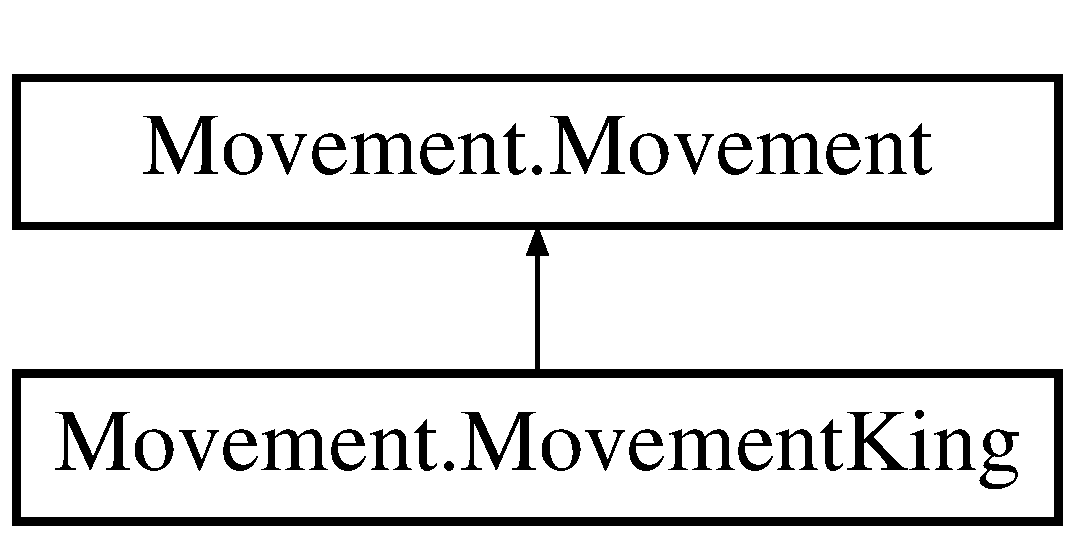
\includegraphics[height=2.000000cm]{class_movement_1_1_movement_king}
\end{center}
\end{figure}
\subsection*{Public Member Functions}
\begin{DoxyCompactItemize}
\item 
\hypertarget{class_movement_1_1_movement_king_a3d79b75a37bc641cb0187220baa83b66}{{\bfseries Movement\-King} (\hyperlink{class_basic___objects_1_1_piece}{Piece}\mbox{[}$\,$\mbox{]}\mbox{[}$\,$\mbox{]} \-\_\-pieces, \hyperlink{class_basic___objects_1_1_piece}{Piece} \-\_\-piece, int \-\_\-x, int \-\_\-y)}\label{class_movement_1_1_movement_king_a3d79b75a37bc641cb0187220baa83b66}

\item 
Array\-List$<$ \hyperlink{class_basic___objects_1_1_position}{Position} $>$ \hyperlink{class_movement_1_1_movement_king_a0ccce7ab8396ee16caf582795f04241f}{check\-King} ()
\end{DoxyCompactItemize}
\subsection*{Additional Inherited Members}


\subsection{Detailed Description}
\hyperlink{class_movement_1_1_movement_rock}{Movement\-Rock} , control the Movements of the King \begin{DoxyAuthor}{Author}
Ignacio Ferrero 
\end{DoxyAuthor}


\subsection{Member Function Documentation}
\hypertarget{class_movement_1_1_movement_king_a0ccce7ab8396ee16caf582795f04241f}{\index{Movement\-::\-Movement\-King@{Movement\-::\-Movement\-King}!check\-King@{check\-King}}
\index{check\-King@{check\-King}!Movement::MovementKing@{Movement\-::\-Movement\-King}}
\subsubsection[{check\-King}]{\setlength{\rightskip}{0pt plus 5cm}Array\-List$<${\bf Position}$>$ Movement.\-Movement\-King.\-check\-King (
\begin{DoxyParamCaption}
{}
\end{DoxyParamCaption}
)}}\label{class_movement_1_1_movement_king_a0ccce7ab8396ee16caf582795f04241f}
Gives back every available \hyperlink{class_movement_1_1_movement}{Movement} that the King has checks if the 8 available option the King has 

The documentation for this class was generated from the following file\-:\begin{DoxyCompactItemize}
\item 
src/\-Movement/Movement\-King.\-java\end{DoxyCompactItemize}

\hypertarget{class_movement_test_1_1_movement_king_test}{\section{Movement\-Test.\-Movement\-King\-Test Class Reference}
\label{class_movement_test_1_1_movement_king_test}\index{Movement\-Test.\-Movement\-King\-Test@{Movement\-Test.\-Movement\-King\-Test}}
}
\subsection*{Public Member Functions}
\begin{DoxyCompactItemize}
\item 
\hypertarget{class_movement_test_1_1_movement_king_test_a581051c42689c090d7c0febaf860f1ec}{void {\bfseries test\-Check\-King} ()}\label{class_movement_test_1_1_movement_king_test_a581051c42689c090d7c0febaf860f1ec}

\item 
\hypertarget{class_movement_test_1_1_movement_king_test_a56fec250729567b517cf5edb9858e52a}{void {\bfseries create\-Piece\-Correct} ()}\label{class_movement_test_1_1_movement_king_test_a56fec250729567b517cf5edb9858e52a}

\item 
\hypertarget{class_movement_test_1_1_movement_king_test_abec85d36db77e84c1f8ad1d3ff45392b}{void {\bfseries create\-Piece\-Incorrect} ()}\label{class_movement_test_1_1_movement_king_test_abec85d36db77e84c1f8ad1d3ff45392b}

\item 
\hypertarget{class_movement_test_1_1_movement_king_test_a52a4c793e306d3990300083b931185b0}{void {\bfseries initialize} ()}\label{class_movement_test_1_1_movement_king_test_a52a4c793e306d3990300083b931185b0}

\end{DoxyCompactItemize}


The documentation for this class was generated from the following file\-:\begin{DoxyCompactItemize}
\item 
src/\-Movement\-Test/Movement\-King\-Test.\-java\end{DoxyCompactItemize}

\hypertarget{class_movement_1_1_movement_knight}{\section{Movement.\-Movement\-Knight Class Reference}
\label{class_movement_1_1_movement_knight}\index{Movement.\-Movement\-Knight@{Movement.\-Movement\-Knight}}
}
Inheritance diagram for Movement.\-Movement\-Knight\-:\begin{figure}[H]
\begin{center}
\leavevmode
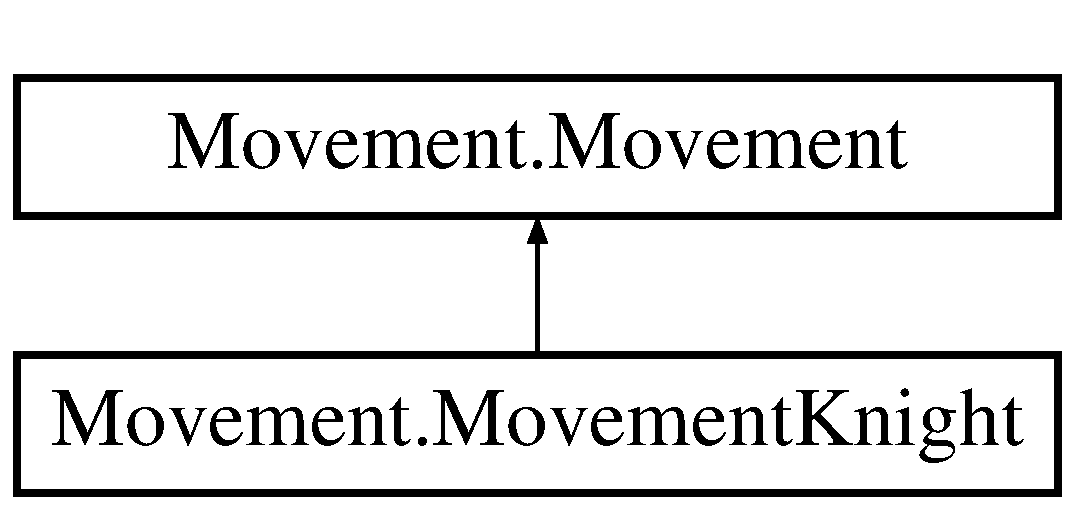
\includegraphics[height=2.000000cm]{class_movement_1_1_movement_knight}
\end{center}
\end{figure}
\subsection*{Public Member Functions}
\begin{DoxyCompactItemize}
\item 
\hypertarget{class_movement_1_1_movement_knight_afa9d052ef6a838d188f1a0a0468fc44c}{{\bfseries Movement\-Knight} (\hyperlink{class_basic___objects_1_1_piece}{Piece}\mbox{[}$\,$\mbox{]}\mbox{[}$\,$\mbox{]} \-\_\-pieces, \hyperlink{class_basic___objects_1_1_piece}{Piece} \-\_\-piece, int \-\_\-x, int \-\_\-y)}\label{class_movement_1_1_movement_knight_afa9d052ef6a838d188f1a0a0468fc44c}

\item 
Array\-List$<$ \hyperlink{class_basic___objects_1_1_position}{Position} $>$ \hyperlink{class_movement_1_1_movement_knight_aa8d179cb6c161d45aa173985d67ade65}{check\-Knight} ()
\end{DoxyCompactItemize}
\subsection*{Additional Inherited Members}


\subsection{Detailed Description}
\hyperlink{class_movement_1_1_movement_rock}{Movement\-Rock} , control the Movements of the Knight \begin{DoxyAuthor}{Author}
Ignacio Ferrero 
\end{DoxyAuthor}


\subsection{Member Function Documentation}
\hypertarget{class_movement_1_1_movement_knight_aa8d179cb6c161d45aa173985d67ade65}{\index{Movement\-::\-Movement\-Knight@{Movement\-::\-Movement\-Knight}!check\-Knight@{check\-Knight}}
\index{check\-Knight@{check\-Knight}!Movement::MovementKnight@{Movement\-::\-Movement\-Knight}}
\subsubsection[{check\-Knight}]{\setlength{\rightskip}{0pt plus 5cm}Array\-List$<${\bf Position}$>$ Movement.\-Movement\-Knight.\-check\-Knight (
\begin{DoxyParamCaption}
{}
\end{DoxyParamCaption}
)}}\label{class_movement_1_1_movement_knight_aa8d179cb6c161d45aa173985d67ade65}
Gives back every available \hyperlink{class_movement_1_1_movement}{Movement} that the Knight has checks if the 8 available option the Knight has 

The documentation for this class was generated from the following file\-:\begin{DoxyCompactItemize}
\item 
src/\-Movement/Movement\-Knight.\-java\end{DoxyCompactItemize}

\hypertarget{class_movement_test_1_1_movement_knight_test}{\section{Movement\-Test.\-Movement\-Knight\-Test Class Reference}
\label{class_movement_test_1_1_movement_knight_test}\index{Movement\-Test.\-Movement\-Knight\-Test@{Movement\-Test.\-Movement\-Knight\-Test}}
}
\subsection*{Public Member Functions}
\begin{DoxyCompactItemize}
\item 
\hypertarget{class_movement_test_1_1_movement_knight_test_a161801a94314b220f337ebfd482a5644}{void {\bfseries test\-Check\-Knight} ()}\label{class_movement_test_1_1_movement_knight_test_a161801a94314b220f337ebfd482a5644}

\item 
\hypertarget{class_movement_test_1_1_movement_knight_test_a295fa2dc83434b03156dea0bbf30a6ad}{void {\bfseries create\-Piece\-Correct} ()}\label{class_movement_test_1_1_movement_knight_test_a295fa2dc83434b03156dea0bbf30a6ad}

\item 
\hypertarget{class_movement_test_1_1_movement_knight_test_a9e9a1fe33f3d4389457eb4e51a702247}{void {\bfseries create\-Piece\-Incorrect} ()}\label{class_movement_test_1_1_movement_knight_test_a9e9a1fe33f3d4389457eb4e51a702247}

\item 
\hypertarget{class_movement_test_1_1_movement_knight_test_aef515bbfbed8a8dae7acab3c03729ba6}{void {\bfseries initialize} ()}\label{class_movement_test_1_1_movement_knight_test_aef515bbfbed8a8dae7acab3c03729ba6}

\end{DoxyCompactItemize}


The documentation for this class was generated from the following file\-:\begin{DoxyCompactItemize}
\item 
src/\-Movement\-Test/Movement\-Knight\-Test.\-java\end{DoxyCompactItemize}

\hypertarget{class_movement_1_1_movement_pawn}{\section{Movement.\-Movement\-Pawn Class Reference}
\label{class_movement_1_1_movement_pawn}\index{Movement.\-Movement\-Pawn@{Movement.\-Movement\-Pawn}}
}
Inheritance diagram for Movement.\-Movement\-Pawn\-:\begin{figure}[H]
\begin{center}
\leavevmode
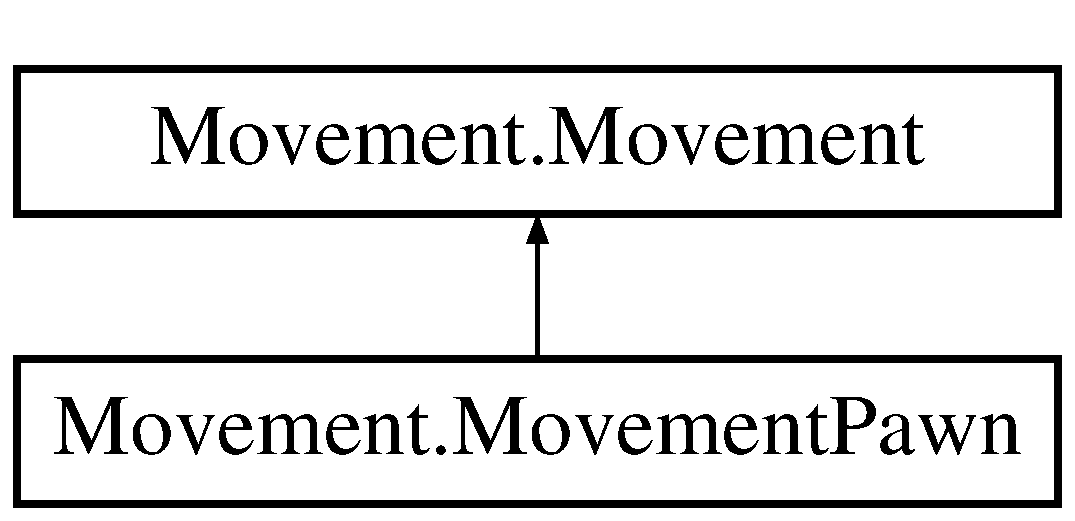
\includegraphics[height=2.000000cm]{class_movement_1_1_movement_pawn}
\end{center}
\end{figure}
\subsection*{Public Member Functions}
\begin{DoxyCompactItemize}
\item 
\hypertarget{class_movement_1_1_movement_pawn_abeb808553b58fa56862b8d9a0485d8fc}{{\bfseries Movement\-Pawn} (\hyperlink{class_basic___objects_1_1_piece}{Piece}\mbox{[}$\,$\mbox{]}\mbox{[}$\,$\mbox{]} \-\_\-pieces, \hyperlink{class_basic___objects_1_1_piece}{Piece} \-\_\-piece, int \-\_\-x, int \-\_\-y)}\label{class_movement_1_1_movement_pawn_abeb808553b58fa56862b8d9a0485d8fc}

\item 
Array\-List$<$ \hyperlink{class_basic___objects_1_1_position}{Position} $>$ \hyperlink{class_movement_1_1_movement_pawn_a04abde45508cbc1ba288aabc91f3a5ab}{check\-Pawn} ()
\end{DoxyCompactItemize}
\subsection*{Additional Inherited Members}


\subsection{Detailed Description}
\hyperlink{class_movement_1_1_movement_pawn}{Movement\-Pawn} , control the Movements of the Pawn

\begin{DoxyAuthor}{Author}
Ignacio Ferrero 
\end{DoxyAuthor}


\subsection{Member Function Documentation}
\hypertarget{class_movement_1_1_movement_pawn_a04abde45508cbc1ba288aabc91f3a5ab}{\index{Movement\-::\-Movement\-Pawn@{Movement\-::\-Movement\-Pawn}!check\-Pawn@{check\-Pawn}}
\index{check\-Pawn@{check\-Pawn}!Movement::MovementPawn@{Movement\-::\-Movement\-Pawn}}
\subsubsection[{check\-Pawn}]{\setlength{\rightskip}{0pt plus 5cm}Array\-List$<${\bf Position}$>$ Movement.\-Movement\-Pawn.\-check\-Pawn (
\begin{DoxyParamCaption}
{}
\end{DoxyParamCaption}
)}}\label{class_movement_1_1_movement_pawn_a04abde45508cbc1ba288aabc91f3a5ab}
Gives back every available \hyperlink{class_movement_1_1_movement}{Movement} that the Pawn has in an Array of Positions 

The documentation for this class was generated from the following file\-:\begin{DoxyCompactItemize}
\item 
src/\-Movement/Movement\-Pawn.\-java\end{DoxyCompactItemize}

\hypertarget{class_movement_test_1_1_movement_pawn_test}{\section{Movement\-Test.\-Movement\-Pawn\-Test Class Reference}
\label{class_movement_test_1_1_movement_pawn_test}\index{Movement\-Test.\-Movement\-Pawn\-Test@{Movement\-Test.\-Movement\-Pawn\-Test}}
}
\subsection*{Public Member Functions}
\begin{DoxyCompactItemize}
\item 
\hypertarget{class_movement_test_1_1_movement_pawn_test_a15d16d880df29ebdcebd7cfa84d3beda}{void {\bfseries test\-Check\-Pawn} ()}\label{class_movement_test_1_1_movement_pawn_test_a15d16d880df29ebdcebd7cfa84d3beda}

\item 
\hypertarget{class_movement_test_1_1_movement_pawn_test_a54271572194dd257866c416878b5e55a}{void {\bfseries create\-Piece\-Correct} ()}\label{class_movement_test_1_1_movement_pawn_test_a54271572194dd257866c416878b5e55a}

\item 
\hypertarget{class_movement_test_1_1_movement_pawn_test_abd01daf4dbc21f245bc1c9b1405c3595}{void {\bfseries create\-Piece\-Incorrect} ()}\label{class_movement_test_1_1_movement_pawn_test_abd01daf4dbc21f245bc1c9b1405c3595}

\item 
\hypertarget{class_movement_test_1_1_movement_pawn_test_a5fe1d5869ae93a11ce0956da920a6b4d}{void {\bfseries initialize} ()}\label{class_movement_test_1_1_movement_pawn_test_a5fe1d5869ae93a11ce0956da920a6b4d}

\end{DoxyCompactItemize}


The documentation for this class was generated from the following file\-:\begin{DoxyCompactItemize}
\item 
src/\-Movement\-Test/Movement\-Pawn\-Test.\-java\end{DoxyCompactItemize}

\hypertarget{class_movement_1_1_movement_rock}{\section{Movement.\-Movement\-Rock Class Reference}
\label{class_movement_1_1_movement_rock}\index{Movement.\-Movement\-Rock@{Movement.\-Movement\-Rock}}
}
Inheritance diagram for Movement.\-Movement\-Rock\-:\begin{figure}[H]
\begin{center}
\leavevmode
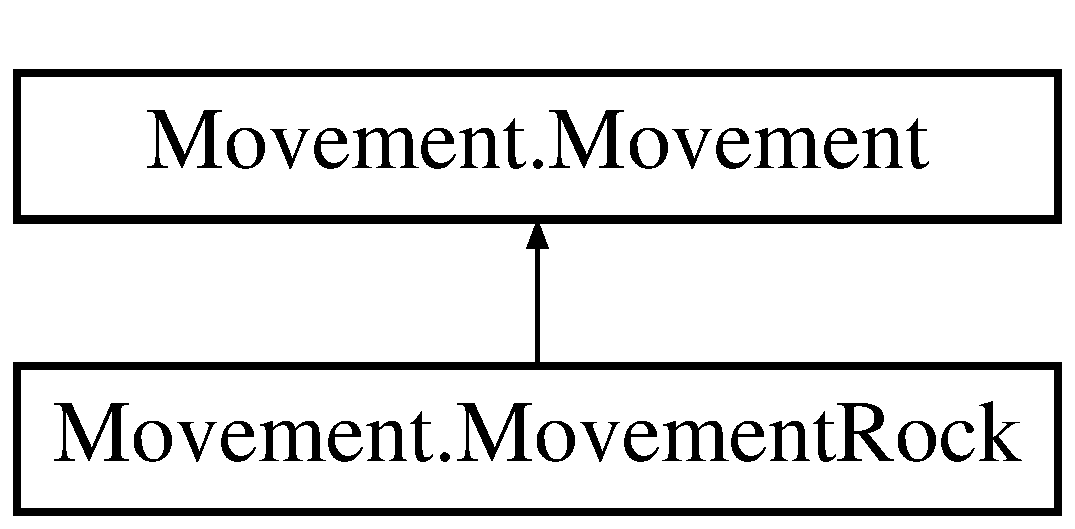
\includegraphics[height=2.000000cm]{class_movement_1_1_movement_rock}
\end{center}
\end{figure}
\subsection*{Public Member Functions}
\begin{DoxyCompactItemize}
\item 
\hypertarget{class_movement_1_1_movement_rock_a1679e753f28043c9478a4d16e8847353}{{\bfseries Movement\-Rock} (\hyperlink{class_basic___objects_1_1_piece}{Piece}\mbox{[}$\,$\mbox{]}\mbox{[}$\,$\mbox{]} \-\_\-pieces, \hyperlink{class_basic___objects_1_1_piece}{Piece} \-\_\-piece, int \-\_\-x, int \-\_\-y)}\label{class_movement_1_1_movement_rock_a1679e753f28043c9478a4d16e8847353}

\item 
Array\-List$<$ \hyperlink{class_basic___objects_1_1_position}{Position} $>$ \hyperlink{class_movement_1_1_movement_rock_a8a640abbb5f0d5c61018fc819c5a9e0b}{check\-Rook} ()
\end{DoxyCompactItemize}
\subsection*{Protected Member Functions}
\begin{DoxyCompactItemize}
\item 
boolean\mbox{[}$\,$\mbox{]} \hyperlink{class_movement_1_1_movement_rock_a9be70803c1f6e816295c11a341e04f15}{check\-Movement} (int i, int j)
\end{DoxyCompactItemize}


\subsection{Detailed Description}
\hyperlink{class_movement_1_1_movement_rock}{Movement\-Rock} , control the Movements of the Rock \begin{DoxyAuthor}{Author}
Ignacio Ferrero 
\end{DoxyAuthor}


\subsection{Member Function Documentation}
\hypertarget{class_movement_1_1_movement_rock_a9be70803c1f6e816295c11a341e04f15}{\index{Movement\-::\-Movement\-Rock@{Movement\-::\-Movement\-Rock}!check\-Movement@{check\-Movement}}
\index{check\-Movement@{check\-Movement}!Movement::MovementRock@{Movement\-::\-Movement\-Rock}}
\subsubsection[{check\-Movement}]{\setlength{\rightskip}{0pt plus 5cm}boolean \mbox{[}$\,$\mbox{]} Movement.\-Movement\-Rock.\-check\-Movement (
\begin{DoxyParamCaption}
\item[{int}]{i, }
\item[{int}]{j}
\end{DoxyParamCaption}
)\hspace{0.3cm}{\ttfamily [protected]}}}\label{class_movement_1_1_movement_rock_a9be70803c1f6e816295c11a341e04f15}
Returns the boolean vector mentioned above checks if it is empty then add the position if not look if its from another color, set boolean\mbox{[}1\mbox{]} to false piece found \hypertarget{class_movement_1_1_movement_rock_a8a640abbb5f0d5c61018fc819c5a9e0b}{\index{Movement\-::\-Movement\-Rock@{Movement\-::\-Movement\-Rock}!check\-Rook@{check\-Rook}}
\index{check\-Rook@{check\-Rook}!Movement::MovementRock@{Movement\-::\-Movement\-Rock}}
\subsubsection[{check\-Rook}]{\setlength{\rightskip}{0pt plus 5cm}Array\-List$<${\bf Position}$>$ Movement.\-Movement\-Rock.\-check\-Rook (
\begin{DoxyParamCaption}
{}
\end{DoxyParamCaption}
)}}\label{class_movement_1_1_movement_rock_a8a640abbb5f0d5c61018fc819c5a9e0b}
Gives back every available \hyperlink{class_movement_1_1_movement}{Movement} that the Rock has in an Array of Positions 

The documentation for this class was generated from the following file\-:\begin{DoxyCompactItemize}
\item 
src/\-Movement/Movement\-Rock.\-java\end{DoxyCompactItemize}

\hypertarget{class_basic___objects_1_1_piece}{\section{Basic\-\_\-\-Objects.\-Piece Class Reference}
\label{class_basic___objects_1_1_piece}\index{Basic\-\_\-\-Objects.\-Piece@{Basic\-\_\-\-Objects.\-Piece}}
}
\subsection*{Public Member Functions}
\begin{DoxyCompactItemize}
\item 
\hypertarget{class_basic___objects_1_1_piece_a8a77d01c5f20edfba9c6a6b7a329ca74}{{\bfseries Piece} (int \-\_\-type, boolean \-\_\-color)}\label{class_basic___objects_1_1_piece_a8a77d01c5f20edfba9c6a6b7a329ca74}

\item 
\hypertarget{class_basic___objects_1_1_piece_a913fe893938642e2634b299289236167}{void {\bfseries set\-Type} (int \-\_\-type)}\label{class_basic___objects_1_1_piece_a913fe893938642e2634b299289236167}

\item 
\hypertarget{class_basic___objects_1_1_piece_af5455dcbe84c08a0afe7ab8cf56add21}{void {\bfseries set\-Color} (boolean \-\_\-color)}\label{class_basic___objects_1_1_piece_af5455dcbe84c08a0afe7ab8cf56add21}

\item 
\hypertarget{class_basic___objects_1_1_piece_a9e5be2fca010d89ecb6dfaf91a0eb058}{void {\bfseries set\-Position} (\hyperlink{class_basic___objects_1_1_position}{Position} \-\_\-position)}\label{class_basic___objects_1_1_piece_a9e5be2fca010d89ecb6dfaf91a0eb058}

\item 
\hypertarget{class_basic___objects_1_1_piece_a64f78783deb89a041d344bfb9d0b3d0a}{boolean {\bfseries get\-Color} ()}\label{class_basic___objects_1_1_piece_a64f78783deb89a041d344bfb9d0b3d0a}

\item 
\hypertarget{class_basic___objects_1_1_piece_acc2175d2a0d7772d5c5f42dd77a816fc}{int {\bfseries get\-Type} ()}\label{class_basic___objects_1_1_piece_acc2175d2a0d7772d5c5f42dd77a816fc}

\end{DoxyCompactItemize}


The documentation for this class was generated from the following file\-:\begin{DoxyCompactItemize}
\item 
src/\-Basic\-\_\-\-Objects/Piece.\-java\end{DoxyCompactItemize}

\hypertarget{class_basic___objects_1_1_player}{\section{Basic\-\_\-\-Objects.\-Player Class Reference}
\label{class_basic___objects_1_1_player}\index{Basic\-\_\-\-Objects.\-Player@{Basic\-\_\-\-Objects.\-Player}}
}
\subsection*{Public Member Functions}
\begin{DoxyCompactItemize}
\item 
\hypertarget{class_basic___objects_1_1_player_af7e6503b73e6881ce72038623245306d}{{\bfseries Player} (boolean \-\_\-logic)}\label{class_basic___objects_1_1_player_af7e6503b73e6881ce72038623245306d}

\item 
\hypertarget{class_basic___objects_1_1_player_afba3554e21a1c306bb99e8f65a73b3f4}{boolean {\bfseries get\-Logic} ()}\label{class_basic___objects_1_1_player_afba3554e21a1c306bb99e8f65a73b3f4}

\item 
\hypertarget{class_basic___objects_1_1_player_a95df7c4b31416cb228711eb4451edf3f}{boolean {\bfseries get\-Check} ()}\label{class_basic___objects_1_1_player_a95df7c4b31416cb228711eb4451edf3f}

\item 
\hypertarget{class_basic___objects_1_1_player_a4fa211cc84a1c48ab219f95bb948ee95}{void {\bfseries set\-Check} ()}\label{class_basic___objects_1_1_player_a4fa211cc84a1c48ab219f95bb948ee95}

\item 
\hypertarget{class_basic___objects_1_1_player_a1bfd2ce47e3d904ee0a3e5d8b540b648}{void {\bfseries set\-Check\-False} ()}\label{class_basic___objects_1_1_player_a1bfd2ce47e3d904ee0a3e5d8b540b648}

\end{DoxyCompactItemize}


The documentation for this class was generated from the following file\-:\begin{DoxyCompactItemize}
\item 
src/\-Basic\-\_\-\-Objects/Player.\-java\end{DoxyCompactItemize}

\hypertarget{class_basic___objects_1_1_position}{\section{Basic\-\_\-\-Objects.\-Position Class Reference}
\label{class_basic___objects_1_1_position}\index{Basic\-\_\-\-Objects.\-Position@{Basic\-\_\-\-Objects.\-Position}}
}
\subsection*{Public Member Functions}
\begin{DoxyCompactItemize}
\item 
\hypertarget{class_basic___objects_1_1_position_aebfc2323eee12f74ec390a24635117d6}{{\bfseries Position} (int \-\_\-x, int \-\_\-y)}\label{class_basic___objects_1_1_position_aebfc2323eee12f74ec390a24635117d6}

\item 
\hypertarget{class_basic___objects_1_1_position_abeb57b2c9f06ea343139f1d23b5d18f4}{void {\bfseries update\-Position} (int \-\_\-x, int \-\_\-y)}\label{class_basic___objects_1_1_position_abeb57b2c9f06ea343139f1d23b5d18f4}

\item 
\hypertarget{class_basic___objects_1_1_position_a6fa4b5005c59bda78470e793a7a13142}{int {\bfseries get\-X} ()}\label{class_basic___objects_1_1_position_a6fa4b5005c59bda78470e793a7a13142}

\item 
\hypertarget{class_basic___objects_1_1_position_a827d50dd8c09eba8eb2aa182bfadf5c2}{int {\bfseries get\-Y} ()}\label{class_basic___objects_1_1_position_a827d50dd8c09eba8eb2aa182bfadf5c2}

\item 
\hypertarget{class_basic___objects_1_1_position_a13be729b959179166226df0a99ea78d6}{boolean {\bfseries check} (\hyperlink{class_basic___objects_1_1_position}{Position} position)}\label{class_basic___objects_1_1_position_a13be729b959179166226df0a99ea78d6}

\end{DoxyCompactItemize}


The documentation for this class was generated from the following file\-:\begin{DoxyCompactItemize}
\item 
src/\-Basic\-\_\-\-Objects/Position.\-java\end{DoxyCompactItemize}

%--- End generated contents ---

% Index
\newpage
\phantomsection
\addcontentsline{toc}{chapter}{Index}
\printindex

\end{document}
